\scanpage{32}

\margin{\begin{minipage}{1.5cm}
\begin{tikzpicture}[overlay,baseline=0pt]
\draw (0.77,0.36) .. controls (0.74,0.78) and (0.21,0.84) .. (0.06,0.36)
 .. controls (-0.08,-0.01) and (0.07,-0.40) .. (0.38,-0.37)
 .. controls (0.65,-0.34) and (0.84,-0.05) .. (0.80,0.21);
\draw (0.94,-0.43) .. controls (1.12,-0.73) and (0.89,-1.11) .. (0.56,-1.10)
 .. controls (0.24,-1.08) and (0.12,-0.72) .. (0.32,-0.48)
 .. controls (0.49,-0.23) and (0.82,-0.22) .. (0.90,-0.46);
\end{tikzpicture}
\(\varphi^{(\ell)}\)\\[0.5em]
\hspace*{0.25cm}\({}_{\ell^\nu}P\)
\end{minipage}}
\[
(2.2.4)\qquad
\deleted{\unsure{\$}}\phi^{(\ell)}_{\inserted{\xi}}\deleted{\unsure{\$}}
=(\phi^{\ell^\nu}_{\inserted{\xi}})_{\nu\geq0},
\quad\text{où}\quad
\phi^{\ell^\nu}_{\inserted{\xi}}:{}_{\ell^\nu}P\times{}_{\ell^\nu}Q\longrightarrow G.
\]
Les diagrammes \rule{0pt}{4ex}\makebox[0pt][l]{\hspace*{-2em}\raisebox{2.4ex}{\inserted{commutatifs}}}\makebox[0pt][l]{
\begin{tikzpicture}[overlay,baseline,x=1em,y=1ex]\draw (-.40,-.55) .. controls (-.72,.45) and (-.42,1.2) .. (.35,1.25) .. controls (1.8,1.6) and (3.8,1.2) .. (4.35,1.40) .. controls (5.2,1.9) and (5.35,2.7) .. (5.05,3.25);\end{tikzpicture}}\deleted{déduits} de (2.2.2) en y faisant $n=\ell^\nu$, $n'=\ell^{\nu'}$, pour $\nu'\geq\nu$, montrent que $\phi^{(\ell)}_{\inserted{\xi}}$ peut être interprété comme un accouplement de \deleted{pro-groupes} systèmes projectifs de groupes
\[
(2.2.5)\qquad
\phi^{(\ell)}_{\inserted{\xi}}:T_\ell(P)\times T_\ell(Q)\longrightarrow T_\ell(G),
\]
où, pour un \deleted{\unsure{G}}groupe $M$ de $T$ et un nombre premier $\ell$, on désigne par
\[
T_\ell(M)=({}_{\ell^\nu}M)_{\nu\geq0}
\]
le système projectif des ${}_{\ell^\nu}M$. L'accouplement \deleted{\unsure{\$}} (2.2.5) est encore appelé \uline{l'accouplement} $\ell$-\uline{adique associé à} $\xi$ (ou à la biextension $E$ de classe $\xi$). Pour $\xi$ variable, on obtient un homomorphisme canonique
\[
(2.2.6)\qquad
\operatorname{Biext}^{\inserted{1}}(P,Q;G)\longrightarrow
\operatorname{Hom}(T_\ell(P)\otimes T_\ell(Q),T_\ell(G)).
\]
On notera que les homomorphismes (2.1.2) sont \uline{fonctoriels} en $P,Q,G$
\par\noindent
\begin{tikzpicture}[overlay,baseline=0pt]
\draw (-0.78,-0.17) .. controls (-0.20,-0.24) and (0.57,-0.09) .. (1.37,-0.12) .. controls (1.43,-0.12) and (1.43,-0.08) .. (1.41,-0.03);
\draw (-0.91,-0.36) .. controls (-0.28,-0.44) and (0.78,-0.37) .. (1.57,-0.32);
\end{tikzpicture}
(pour $n$ fixé), d'où on déduit qu'il en est de même de (2.2.6).

2.3. \deleted{On peut regarder} La compatibilité (2.2.2) permet de retrouver $\phi^n_{\inserted{\xi}}$ connaissant $\phi^{n'}_{\inserted{\xi}}$, pourvu que ${}_{n'}Q\xrightarrow{m}{}_nQ$ \inserted{soit} un épimorphisme, --- \deleted{(NB l'h} condition satisfaite, comme il est bien connu, si $nQ=Q$. En effet, comme ${}_{n'}P\xrightarrow{m}{}_nP$ est aussi un épimorphisme, $\phi^n_{\inserted{\xi}}$ se déduit \deleted{\unsure{de}}alors de $\phi^{n'}_{\inserted{\xi}}$ par passage au quotient. On peut cependant \rule{0pt}{4ex}\makebox[0pt][l]{\raisebox{2.4ex}{\inserted{donner}}}\makebox[0pt][l]{\begin{tikzpicture}[overlay,baseline,x=1em,y=1ex]\draw[line width=.45pt] (-.25,-.55) -- (-.31,1.02) .. controls (-.28,1.60) and (.0,1.56) .. (.55,1.53) .. controls (1.45,1.58) and (2.60,1.22) .. (3.25,1.71) .. controls (3.65,2.0) and (3.64,2.63) .. (3.45,2.91);\draw[line width=.25pt] (-.17,-.75) .. controls (-.42,.45) and (.10,1.48) .. (.62,1.30) .. controls (1.6,1.13) and (2.90,1.03) .. (3.56,2.18);\end{tikzpicture}} une compatibilité légèrement plus précise que (2.2.2), qui permet d\deleted{e}'exprimer $\phi^n$ en termes de $\phi^{n'}$ sans aucune restriction sur $Q$, par la commutativité de

(2.3.1)
\diagram{\begin{tikzcd}[ampersand replacement=\&,column sep=small,row sep=large]
{}_{n'}P \arrow[d,"m"] \& \times \& {}_nQ \arrow[d,"\mathrm{id}"] \arrow[rr,"{\phi^{n'}_{\inserted{\xi}}|_{{}_{n'}P\times{}_nQ}}"] \& \& {}_nG \arrow[d,"\mathrm{id}"]\\
{}_{\deleted{\unsure{m|n}}n}P \& \times \& {}_nQ \arrow[rr,"\phi^n_{\inserted{\xi}}"] \& \& {}_nG
\end{tikzcd}},

en formules
\[
(2.3.2)\qquad
\phi^n_{\inserted{\xi}}(mx,y)=\phi^{n'}_{\inserted{\xi}}(x,y)
\qquad(x\in{}_{n'}P(S),\ y\in{}_nQ(S)).
\]
Cette formule implique évidemment la commutativité de (2.2.2), qui s'écrit en effet
\[
\inserted{(2.3.3)}\qquad
\phi^n_{\inserted{\xi}}(mx,my)=m\phi^{n'}_{\inserted{\xi}}(x,y)
\qquad(x\in{}_{n'}P(S),\ y\in{}_{n'}P(S)),
\]
\margin{31}
